%%%%%%%%%%%%%%%%%%%%%%%%%%%%%%%%%%%%%%%%%
% Beamer Presentation
% LaTeX Template
% Version 1.0 (10/11/12)
%
% This template has been downloaded from:
% http://www.LaTeXTemplates.com
%
% License:
% CC BY-NC-SA 3.0 (http://creativecommons.org/licenses/by-nc-sa/3.0/)
%
%%%%%%%%%%%%%%%%%%%%%%%%%%%%%%%%%%%%%%%%%

%----------------------------------------------------------------------------------------
%	PACKAGES AND THEMES
%----------------------------------------------------------------------------------------

\documentclass{beamer}

\mode<presentation> {

% The Beamer class comes with a number of default slide themes
% which change the colors and layouts of slides. Below this is a list
% of all the themes, uncomment each in turn to see what they look like.

%\usetheme{default}
%\usetheme{AnnArbor}
%\usetheme{Antibes}
%\usetheme{Bergen}
%\usetheme{Berkeley}
%\usetheme{Berlin}
%\usetheme{Boadilla}
%\usetheme{CambridgeUS}
%\usetheme{Copenhagen}
%\usetheme{Darmstadt}
%\usetheme{Dresden}
%\usetheme{Frankfurt}
%\usetheme{Goettingen}
%\usetheme{Hannover}
%\usetheme{Ilmenau}
%\usetheme{JuanLesPins}
%\usetheme{Luebeck}
\usetheme{Madrid}
%\usetheme{Malmoe}
%\usetheme{Marburg}
%\usetheme{Montpellier}
%\usetheme{PaloAlto}
%\usetheme{Pittsburgh}
%\usetheme{Rochester}
%\usetheme{Singapore}
%\usetheme{Szeged}
%\usetheme{Warsaw}

% As well as themes, the Beamer class has a number of color themes
% for any slide theme. Uncomment each of these in turn to see how it
% changes the colors of your current slide theme.

%\usecolortheme{albatross}
%\usecolortheme{beaver}
%\usecolortheme{beetle}
%\usecolortheme{crane}
%\usecolortheme{dolphin}
%\usecolortheme{dove}
%\usecolortheme{fly}
%\usecolortheme{lily}
%\usecolortheme{orchid}
%\usecolortheme{rose}
%\usecolortheme{seagull}
%\usecolortheme{seahorse}
%\usecolortheme{whale}
%\usecolortheme{wolverine}

%\setbeamertemplate{footline} % To remove the footer line in all slides uncomment this line
%\setbeamertemplate{footline}[page number] % To replace the footer line in all slides with a simple slide count uncomment this line

%\setbeamertemplate{navigation symbols}{} % To remove the navigation symbols from the bottom of all slides uncomment this line
}
\graphicspath{{Figures/}}
\usepackage{graphicx} % Allows including images
\usepackage{booktabs} % Allows the use of \toprule, \midrule and \bottomrule in tables

%----------------------------------------------------------------------------------------
%	TITLE PAGE
%----------------------------------------------------------------------------------------

\title[Prob. Conn of USN]{Probabilistic Connectivity of Underwater Sensor Networks} % The short title appears at the bottom of every slide, the full title is only on the title page

\author{Md Asadul Islam} % Your name
\institute[UofA] % Your institution as it will appear on the bottom of every slide, may be shorthand to save space
{
University of Alberta \\ % Your institution for the title page
\medskip
\textit{mdasadul@ualberta.ca} % Your email address
}
\date{\today} % Date, can be changed to a custom date

\begin{document}

\begin{frame}
\titlepage % Print the title page as the first slide
\end{frame}

\begin{frame}
\frametitle{Overview} % Table of contents slide, comment this block out to remove it
\tableofcontents % Throughout your presentation, if you choose to use \section{} and \subsection{} commands, these will automatically be printed on this slide as an overview of your presentation
\end{frame}

%----------------------------------------------------------------------------------------
%	PRESENTATION SLIDES
%----------------------------------------------------------------------------------------

%------------------------------------------------
\section{First Section} % Sections can be created in order to organize your presentation into discrete blocks, all sections and subsections are automatically printed in the table of contents as an overview of the talk
%------------------------------------------------

\subsection{Subsection Example} % A subsection can be created just before a set of slides with a common theme to further break down your presentation into chunks

%------------------------------------------------

\begin{frame}
\frametitle{Why UWSNs?}
UWSNs fuelled by many important underwater sensing applications and services such as

\begin{itemize}
\item \textbf{Scientific applications}: e.g., observing  geological processes on the ocean floor, determining water characteristics, counting or imaging animal life
\item \textbf{Industrial applications}: e.g., monitoring and control of commercial activities, determining routes for underwater cables, monitoring underwater equipment  and pipelines for oil and mineral extraction, and monitoring commercial fisheries
\item \textbf{Military and homeland security applications}: e.g., monitoring and securing port facilities

\item \textbf{Humanitarian applications}: e.g., search and survey missions, disaster prevention tasks, identification of seabed hazards, locating dangerous rocks or shoals, and identifying possible mooring locations
\end{itemize}
\end{frame}

%------------------------------------------------

\begin{frame}

\frametitle{Challenges of the underwater communication channel}
\begin{block}{Radio Communication}
\begin{itemize}
\item suffer strong attenuation in salt water
\item short distances (6-20 m) and low data rates (1 Kbps)
\item require large antennas and high transmission power
\end{itemize}
\end{block}

\begin{block}{Optical Communication}
\begin{itemize}
\item strongly scattered and absorbed underwater
\item  limited to short distances (≤ 40 m)
\end{itemize}
\end{block}

\begin{block}{Acoustic Communication}
\begin{itemize}
\item suffers from attenuation, spreading, and noise 
\item very long delay because of low propagation speed.
\item it is most practical method upto now 
\end{itemize}
\end{block}
\end{frame}

%------------------------------------------------
\begin{frame}
\frametitle{Challenges due to node mobility}
\begin{block}{Static Deployment}
\begin{itemize}
\item nodes attached to underwater ground, anchored buoys, or docks
\item 
\end{itemize}
\end{block}
\begin{block}{Semi-mobile Deployment}
\begin{itemize}
\item nodes attached to a free floating buoy
\item subject to small scale movement 
\end{itemize}
\end{block}
\begin{block}{Mobile Deployment}
\begin{itemize}
\item composed of drifters with self/noself mobile capability
\item are subject to large scale movement
\item maintaining connectivity is important to perform localization, routing etc. 
\end{itemize}
\end{block}
\end{frame}
%------------------------------------------------
\begin{frame}
\frametitle{Kinematic Model}
We note that this area is new to networking researchers where the obtained analytical
results are rooted in the mathematically deep field of fluid dynamics.
\begin{itemize}
\item A particle pathline is a path followed by an individual particle in a flow
\item A \textit{stream} function denoted  by $\psi$ measures the volume flow rate per unit depth.
\item Curves where $\psi$ is constant are called \textit{streamlines}
\end{itemize}
The stream function can be presented \\
\begin{equation}\label{eq:sf}
\psi(x,y,t)=-\tanh{[\frac{y-B(t)\sin(k(x-ct))}{\sqrt{1 + k^2 B^2(t) \cos^2(k(x-ct))}} ]} + cy
\end{equation}
 where $  B(t) = A + \epsilon \cos(\omega t)$  and the x and y velocities are given by
 
 \begin{equation}\label{eq:lf}
\dot{x}=-\frac{\partial \psi}{\partial y} ; \dot{y}=\frac{\partial \psi}{\partial x}
\end{equation}
\end{frame}
%------------------------------------------------
\begin{frame}
\frametitle{}
\begin{figure}[!htb]
\centering
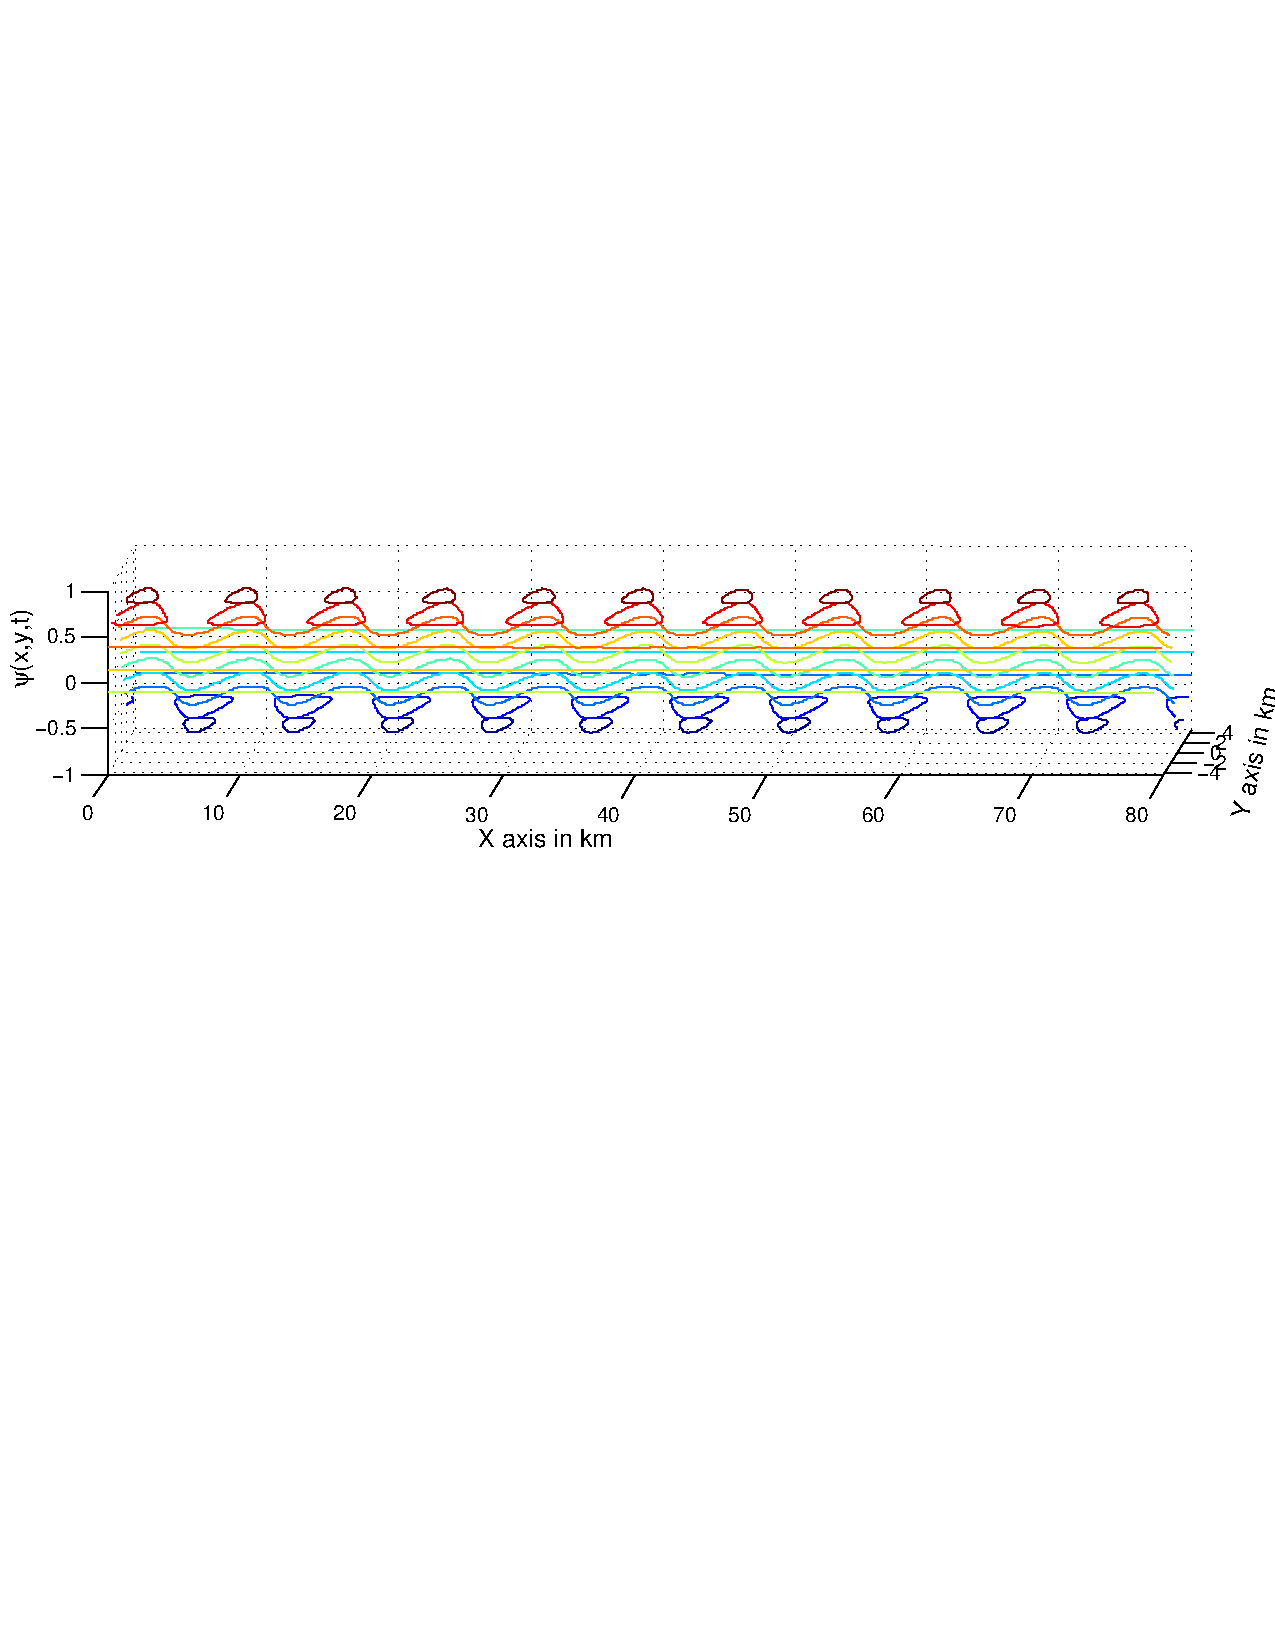
\includegraphics[width=5 in, height=2.2 in]{3D1.pdf}
 \caption{ A 3D plot of stream function \ref{eq:sf}}
 \label{fig:kme3d}
\end{figure}
\end{frame}


%------------------------------------------------
\begin{frame}
\frametitle{Multiple Columns}
\begin{columns}[c] % The "c" option specifies centered vertical alignment while the "t" option is used for top vertical alignment

\column{.45\textwidth} % Left column and width
\textbf{Heading}
\begin{enumerate}
\item Statement
\item Explanation
\item Example
\end{enumerate}

\column{.5\textwidth} % Right column and width
Lorem ipsum dolor sit amet, consectetur adipiscing elit. Integer lectus nisl, ultricies in feugiat rutrum, porttitor sit amet augue. Aliquam ut tortor mauris. Sed volutpat ante purus, quis accumsan dolor.

\end{columns}
\end{frame}

%------------------------------------------------
\section{Second Section}
%------------------------------------------------

\begin{frame}
\frametitle{Table}
\begin{table}
\begin{tabular}{l l l}
\toprule
\textbf{Treatments} & \textbf{Response 1} & \textbf{Response 2}\\
\midrule
Treatment 1 & 0.0003262 & 0.562 \\
Treatment 2 & 0.0015681 & 0.910 \\
Treatment 3 & 0.0009271 & 0.296 \\
\bottomrule
\end{tabular}
\caption{Table caption}
\end{table}
\end{frame}

%------------------------------------------------

\begin{frame}
\frametitle{Theorem}
\begin{theorem}[Mass--energy equivalence]
$E = mc^2$
\end{theorem}
\end{frame}

%------------------------------------------------

\begin{frame}[fragile] % Need to use the fragile option when verbatim is used in the slide
\frametitle{Verbatim}
\begin{example}[Theorem Slide Code]
\begin{verbatim}
\begin{frame}
\frametitle{Theorem}
\begin{theorem}[Mass--energy equivalence]
$E = mc^2$
\end{theorem}
\end{frame}\end{verbatim}
\end{example}
\end{frame}

%------------------------------------------------

\begin{frame}
\frametitle{Figure}
Uncomment the code on this slide to include your own image from the same directory as the template .TeX file.
%\begin{figure}
%\includegraphics[width=0.8\linewidth]{test}
%\end{figure}
\end{frame}

%------------------------------------------------

\begin{frame}[fragile] % Need to use the fragile option when verbatim is used in the slide
\frametitle{Citation}
An example of the \verb|\cite| command to cite within the presentation:\\~

This statement requires citation \cite{p1}.
\end{frame}

%------------------------------------------------

\begin{frame}
\frametitle{References}
\footnotesize{
\begin{thebibliography}{99} % Beamer does not support BibTeX so references must be inserted manually as below
\bibitem[Smith, 2012]{p1} John Smith (2012)
\newblock Title of the publication
\newblock \emph{Journal Name} 12(3), 45 -- 678.
\end{thebibliography}
}
\end{frame}

%------------------------------------------------

\begin{frame}
\Huge{\centerline{The End}}
\end{frame}

%----------------------------------------------------------------------------------------

\end{document} 